\documentclass[uplatex,10pt,a4paper,twocolumn]{jsarticle}
%
\usepackage{amsmath}
\usepackage{bm}
%
\def\diff{\mathrm d}
\def\dd#1#2{\dfrac{\diff #1}{\diff #2}}
\def\pp#1#2{\dfrac{\partial #1}{\partial #2}}
\def\dd2#1#2{\dfrac{\diff^2 #1}{\diff #2^2}}
\def\pp2#1#2{\dfrac{\partial^2 #1}{\partial #2^2}}
%
\usepackage[dvipdfmx]{graphicx, color}
%
\pagestyle{empty}
\usepackage[truedimen,margin=25truemm]{geometry}

\renewcommand{\baselinestretch}{0.9} % 全体の行間調整
\renewcommand{\figurename}{Fig.}
\renewcommand{\tablename}{Tab.}
\usepackage{setspace}

\graphicspath{{../../Figures/gakkai/}}

\begin{document}
\twocolumn[

\begin{center}
{\Large ランダムな接続性を有するネットワークポリマーの緩和挙動}
\end{center}
\begin{flushright}
{\large 東亞合成  $\bigcirc$佐々木裕}
\end{flushright}

%\vspace{1mm}

\begin{center}
{\large Reluxation Characteristics of Network Polymers with random connectivity \\using Molecular Dynamics Simulations}

$\bigcirc$H. Sasaki\\
Toagosei Co., Ltd
\end{center}
\vspace{2mm}

]


\begin{spacing}{0.95}
ABSTRACT: 
Existence of hysteresis is believed to be one of a key to achieve high durability for rubber materials.
For hysteresis cycle, added fillers are known to play an important roll in meso-scale region response against local stress.
% Our question is ``Is there any other mechanism to enhance durability in micro-scale region such as size of polymer chains?''.

``Phantom Network Model'', in which fluctuation of junction point is rather high, seems to be a good candidate for micro-scale energy dissipation.
Employing molecular dynamics simulation method, reluxation characteristics of ``Phantom Network Model'' was investigated.
\end{spacing}

\section{はじめに}

ゴムの大きな破壊靭性の由来については、 ヒステリシスロスのようなエネルギー散逸により亀裂進展が抑制されるという Andrews モデルが提案されている~\cite{Andrews1977}。
ゴムへのフィラーの添加がヒステリシスの主要な発生原因とされ~\cite{Grosch1968}、その発現機構の一つとしてフィラー近傍でのナノキャビティーの開閉も報告されている~\cite{Zhang2013}。
フィラー由来の靭性向上効果はメゾスケール領域の挙動であると考えられているが、このようなエネルギー散逸挙動はメゾスケールでしか発現しないのであろうか?

ゴム弾性の古典的なモデルは、ガウス鎖をストランドとしたネットワークの結節点のミクロな変形がマクロな変形と相似でアフィン変形するとした``Affine Network Model: ANM'' である。%~\cite{Flory1953}。
この古典モデルからの発展形として、結節点の揺らぎに注目しミクロな変形がマクロと異なるとした``Phantom Network Model: PNM''が提案されている~\cite{James1943}。
Flory によれば、メルト状態と同一なストランドのゆらぎを有するランダムネットワークにおいて PNM のふるまいを示すとされている~\cite{Flory1976}。

我々は、この結節点のゆらぎ由来の散逸が、分子鎖描像のようなミクロなスケールでの粘弾性的なエネルギー散逸モデルとなりうるのではないかと考え、これまで検討を進めている。
以前に、規則構造ネットワークをベースとしてユニットセル間における規則性をランダムへと変えることで架橋欠損のないネットワークを作成して PNM を再現できることを報告した。

本報告では、ランダムな接続性を有するネットワークポリマーの緩和挙動について、MD シミュレーションにより検討した結果について報告する。

\section{シミュレーション}
\vspace{-2mm}

ランダムな結合性を有するネットワークを作成し、その平衡状態および一軸伸長時の振る舞いについて、OCTA 上の COGNAC シミュレーターを用いた分子動力学シミュレーションにより評価した。


\subsection{ネットワークモデルの作成}

任意の分岐数$f$($f=3\sim6$)の結節点からなる規則構造を有するネットワークより、以下のアルゴリズムでランダムな結合性を導入した。

\vspace{-2mm}
\begin{enumerate}
\item
実空間での初期構造を体心立方構造の各格子点をストランドでつないだ「八本鎖モデル」として、それに対応するように任意の分岐数のトポロジーモデルを作成(Fig. \ref{fig:topo})。
\item
代数的連結性を指標として連結性を維持しながらストランド交換し、結節点の結合性にランダム性を導入(Fig. \ref{fig:exc})。
\item
トポロジーモデルに対応して実空間の構造作成。
\end{enumerate}

\vspace{-2mm}
\begin{figure}[htb]
	\begin{center}
	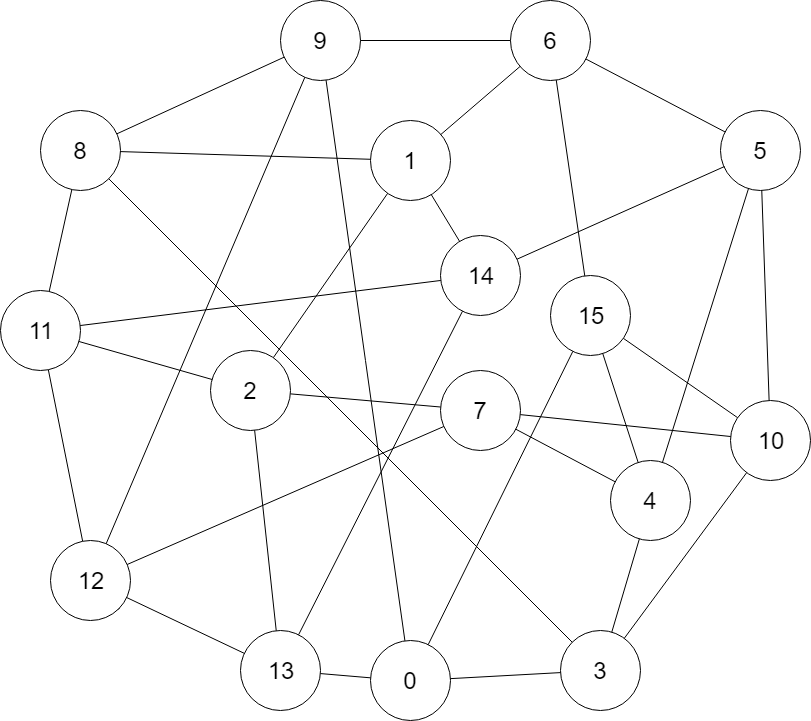
\includegraphics[width=.23\textwidth]{Network.png}
	\caption{Topological NW Model}
	\label{fig:topo}
	\end{center}
\end{figure}

\vspace{-8mm}
\begin{figure}[htb]
	\begin{center}
	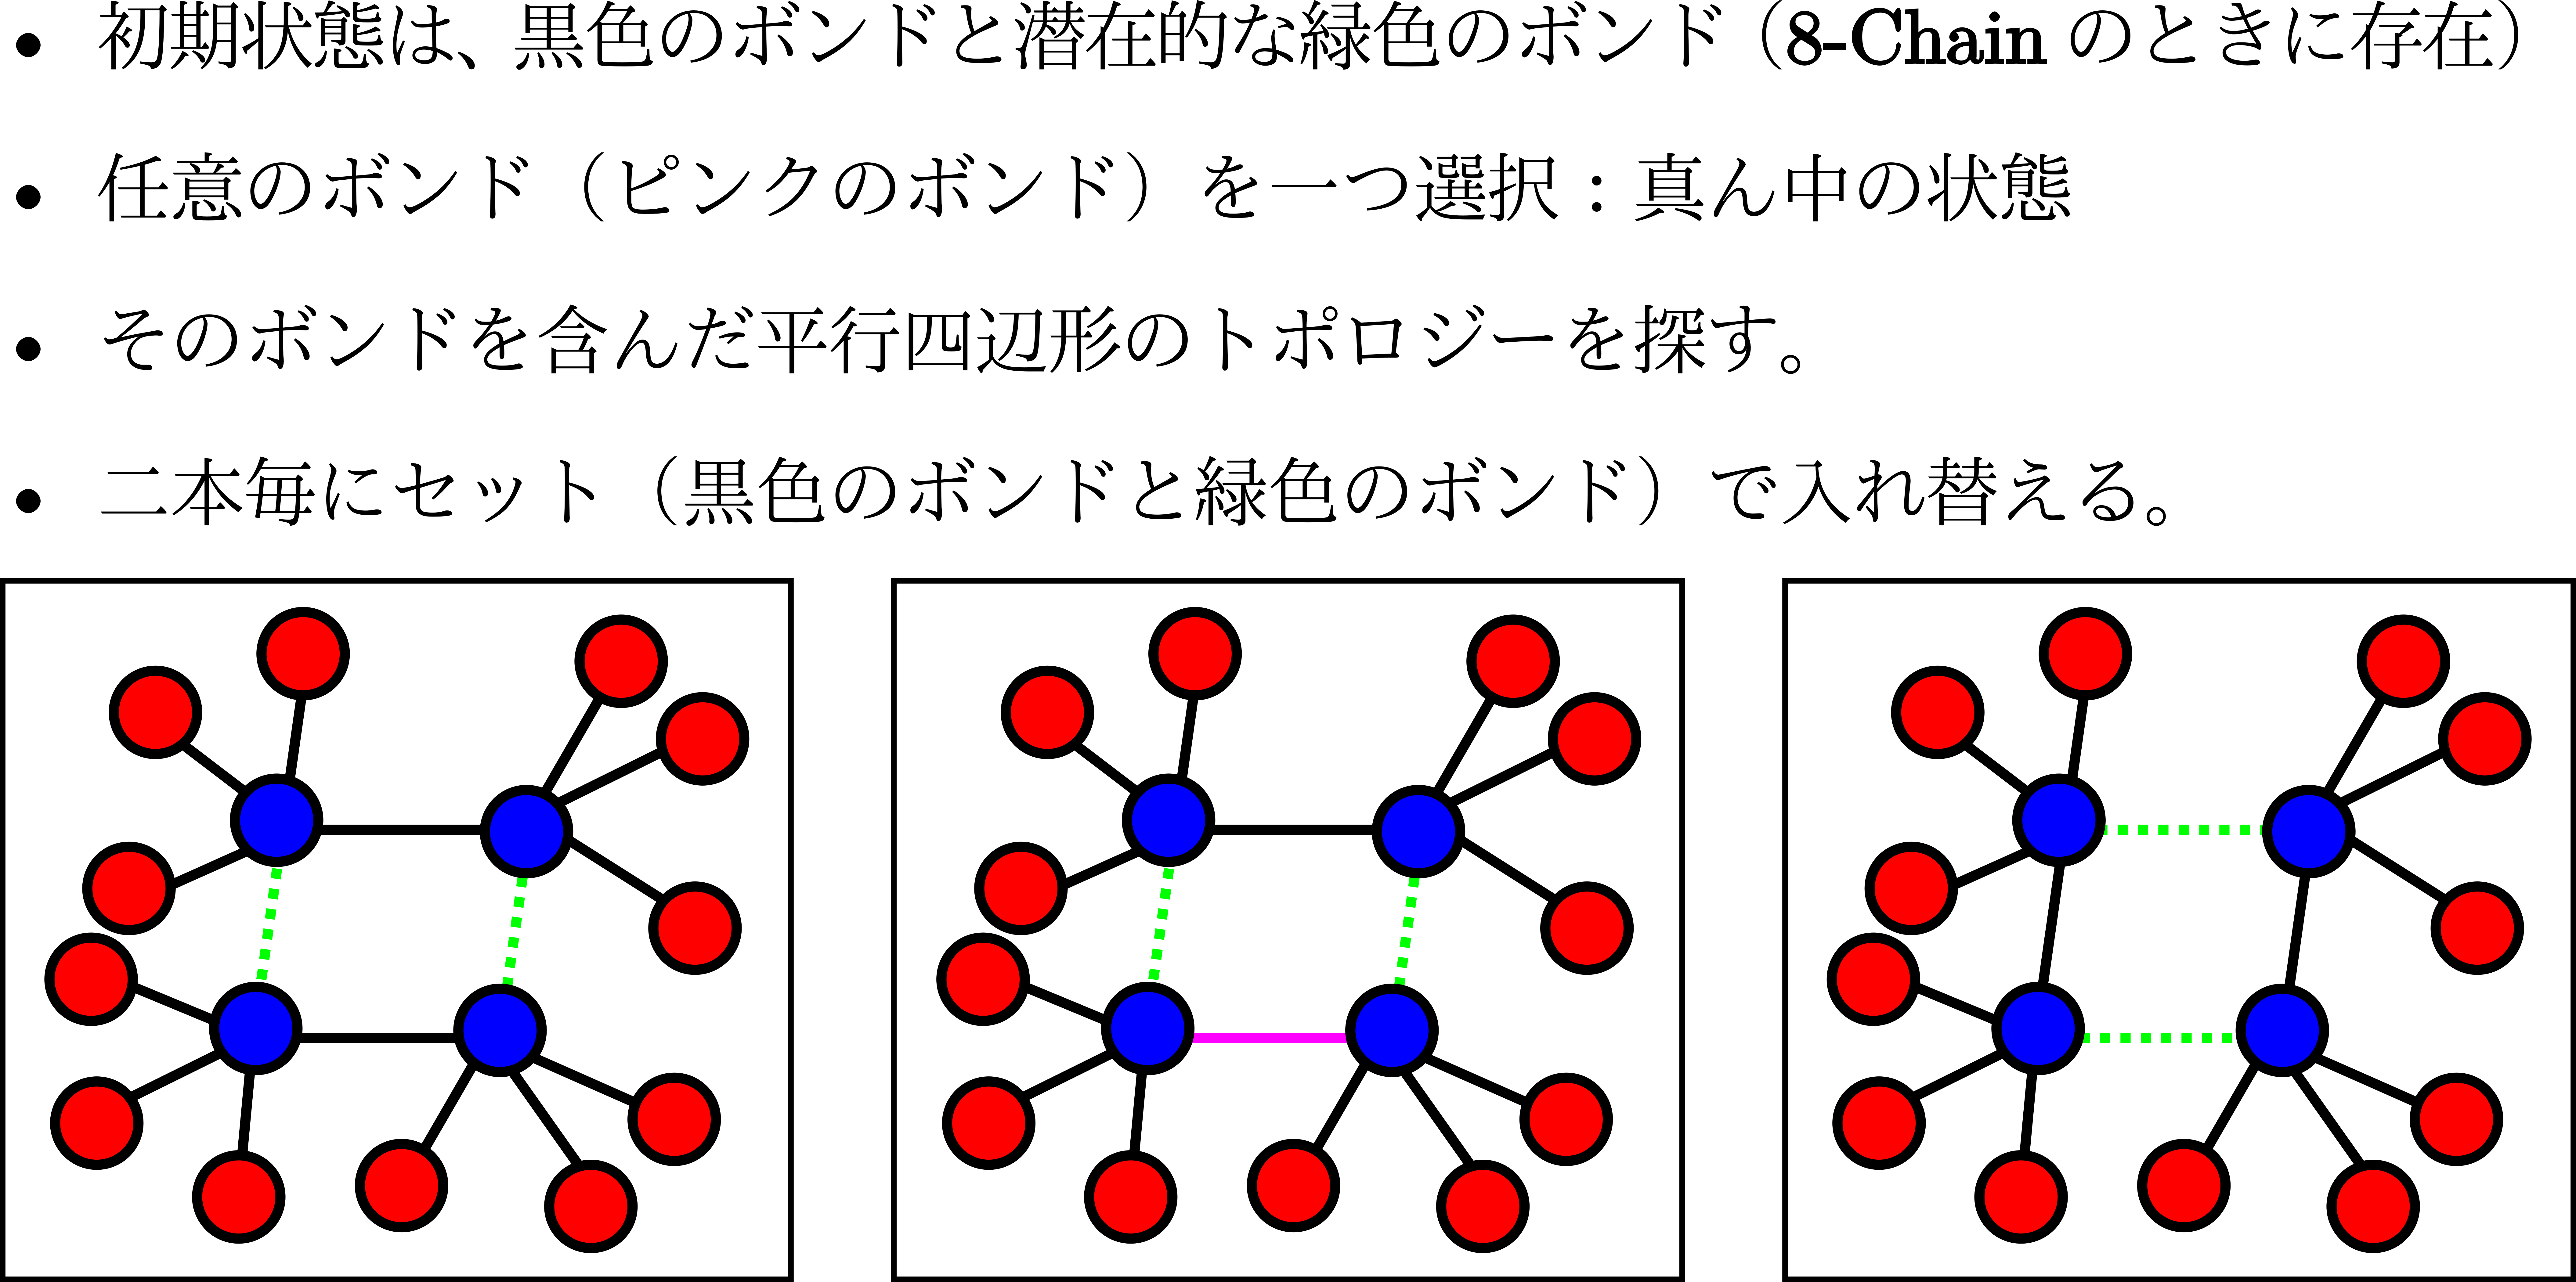
\includegraphics[width=.42\textwidth]{bond_exchg.png}
	\caption{Strand Exchange Procedure}
	\label{fig:exc}
	\end{center}
\end{figure}
\vspace{-5mm}

\subsection{ポテンシャルの設定}
非結合ポテンシャルは、斥力($r_c = 2^{(1/6)}\sigma$)である LJ ポテンシャル $U_{LJ}(r_{ij})$、ボンドポテンシャルには FENE-LJ ポテンシャルを用いて KG 鎖とした。
なお、初期構造の緩和は、Auhl 等の方法~\cite{Auhl2003a} に従い、force-capped-LJ ポテンシャルにより過剰な絡み合いを除外した。


    \section{結果と考察}
    セグメント数 N=48 のストランドを用いて、多重度を変えることで同様な鎖密度 $\nu$ を有する四分岐モデル(多重度 3、4-Chainと表記)を作成し、シミュレーションを行った。
    
    \subsection{ストランドのセグメント間距離 $\langle \bm{R} \rangle$ の分布関数}
    
    四分岐モデルにおけるストランドの長手方向に沿ったセグメント間距離($n=48$ で末端間距離に対応)の分布関数のトラジェクトリーを確認し、部分鎖としての振る舞いは拘束のないメルトポリマー鎖と類似であったが、そのゆらぎは若干低下していることを確認した。
    

    \subsection{$\lambda =2$ からの応力緩和}
    システムの鎖密度を同一としたネットワークを $\lambda =2$ まで迅速に伸長し、応力緩和関数 $G(t)$ を求めた (Fig.\ref{fig:stress_rel})。
    緩和後の弾性率は三分岐の方が低くなったが、いずれも ANM よりも高かった。
    これは、ストランドの絡み合いに起因した Trapped Entanglement により実効的な鎖密度が上昇したと考えられた。

    \begin{figure}[htb]
    \centering
        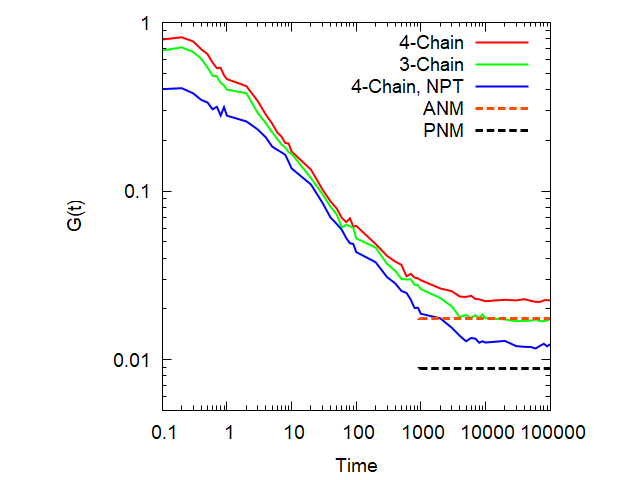
\includegraphics[width=.42\textwidth]{gt_comp_34.png}
    \caption{Stress Relaxations for Uni-axial Step Strain($\lambda=2$)}
    \label{fig:stress_rel}
    \end{figure}

    Primitive Path Analysis (PPA) を行い、多数の絡み合いを確認した (Fig.\ref{fig:ppa})。
    NPT 計算により絡み合いを排除した比較 (4-Chain-NPT) では PPA にて絡み合いが殆どないことが確認でき、弾性率が PNM へと漸近していた。
    
    \begin{figure}[htb]
    \centering
        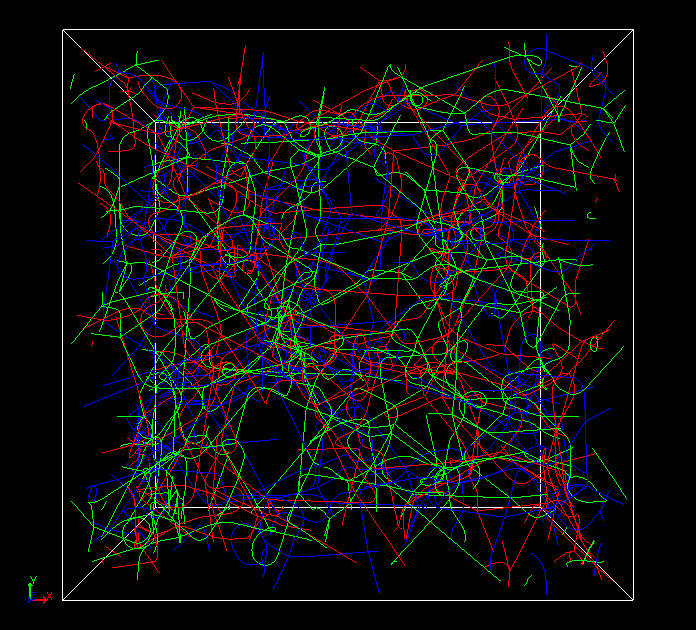
\includegraphics[width=.34\textwidth]{N48_f4_PPA.png}
    \caption{Primitive Path Analysis (PPA) for 4-Chain Model}
    \label{fig:ppa}
    \end{figure}

    この絡み合いの効果については、以前の Rubinstein らの検討結果とよく整合していることが確認できた~\cite{Rubinstein2002}。

    \begin{figure}[htb]
        \centering
            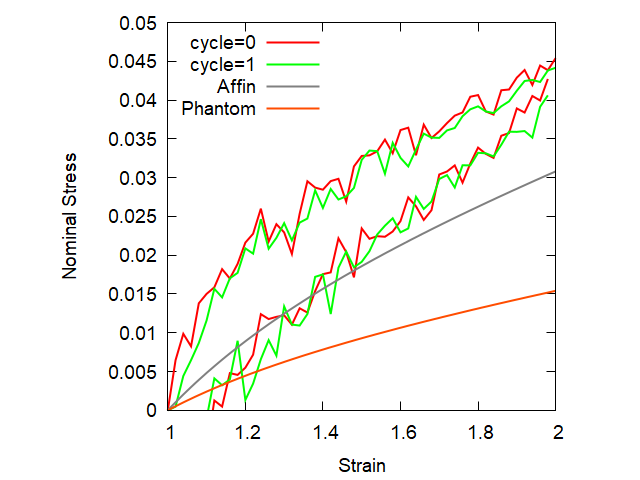
\includegraphics[width=.42\textwidth]{hyst_4Chain.png}
        \caption{Hysteresis Curves for Uni-axial Strain of 4-Chain Model}
        \label{fig:hyst}
        \end{figure}

    \bibliographystyle{../achemso}
    \bibliography{C:/texlive/texmf-local/bibtex/bib/library.bib}
\end{document}